\documentclass{beamer}

% Theme selection
\usetheme{Madrid}
\usecolortheme{default}

% Packages
\usepackage{amsmath}
\usepackage{graphicx}
\usepackage{booktabs}
\usepackage{caption}

% Meta information
\title[Optimasi Portofolio dengan VQE]{Optimasi Portofolio Menggunakan Variational Quantum Eigensolver (VQE)}
\subtitle{Replikasi Studi Kasus pada Saham Teknologi}
\date{\today}

\begin{document}

% Title Slide
\begin{frame}
    \titlepage
\end{frame}

% Outline
\begin{frame}{Outline}
    \tableofcontents
\end{frame}

% Slide 1: Pendahuluan & Latar Belakang
\section{Pendahuluan}
\begin{frame}{Pendahuluan \& Latar Belakang}
    \begin{itemize}
        	\item \textbf{Masalah Optimasi Portofolio:}
        \begin{itemize}
            	\item Menyeimbangkan antara keuntungan (\textit{return}) dan risiko (\textit{risk}).
        \end{itemize}
        \item \textbf{Pendekatan Klasik:}
        \begin{itemize}
            	\item Modern Portfolio Theory (Markowitz).
        \end{itemize}
        \item \textbf{Pendekatan Kuantum:}
        \begin{itemize}
            	\item Menggunakan algoritma hibrid VQE (\textit{Variational Quantum Eigensolver}).
            	\item Bertujuan menyelesaikan masalah kombinatorial yang kompleks.
        \end{itemize}
    \end{itemize}
    
    \vspace{0.5cm}
    \begin{center}
        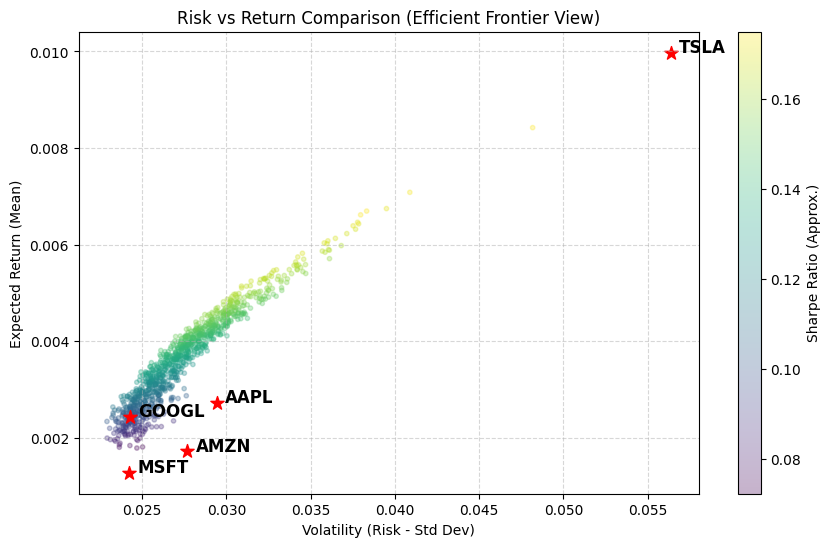
\includegraphics[width=0.35\textwidth]{risk_vs_return.png}
    \end{center}
\end{frame}

% Slide 2: Formulasi Matematis (Markowitz ke QUBO)
\section{Formulasi Matematis}
\begin{frame}{Formulasi Matematis: Markowitz ke QUBO}
    \textbf{1. Fungsi Objektif Awal (Markowitz)}
    \begin{equation*}
        \text{Minimize} \quad w \underbrace{\sum_{i,j} \sigma_{ij} x_i x_j}_{\text{Risk (Variance)}} - (1-w) \underbrace{\sum_i \mu_i x_i}_{\text{Return}}
    \end{equation*}
    \begin{itemize}
        	\item $x_i \in \{0, 1\}$: Variabel biner (pilih aset atau tidak).
        	\item $w$: Parameter penghindaran risiko (\textit{risk aversion}).
    \end{itemize}

    \textbf{2. Constraint (Kendala)}
    \begin{equation*}
        \sum_{i=1}^N x_i = B \quad (\text{Memilih tepat } B \text{ aset})
    \end{equation*}
\end{frame}

\begin{frame}{Formulasi Matematis: Metode Penalti}
    \textbf{3. Metode Penalti (Unconstrained Optimization)}
    Agar dapat diselesaikan dengan VQE, kendala diubah menjadi \textit{penalty term}.
    \begin{equation*}
        \text{Penalty} = P \left( \sum_{i=1}^N x_i - B \right)^2
    \end{equation*}
    
    \textbf{4. Total Cost Function (Hamiltonian)}
    \begin{equation*}
        C(x) = w x^T \Sigma x - (1-w) \mu^T x + P \left( \sum x_i - B \right)^2
    \end{equation*}
\end{frame}

% Slide 3: Mapping ke Hamiltonian Kuantum
\section{Mapping Kuantum}
\begin{frame}{Mapping ke Hamiltonian Kuantum}
    \begin{itemize}
        	\item \textbf{Harus ada cara agar komputer kuantum memahami variabel biner}
        \item Mapping variabel biner $x_i \in \{0, 1\}$ ke operator spin/qubit $Z_i$.
        \item \textbf{Transformasi:}
        \begin{equation*}
            x_i \rightarrow \frac{1-Z_i}{2}
        \end{equation*}
        \item Hasil akhirnya adalah \textbf{Ising Hamiltonian} yang akan diminimalkan energinya oleh VQE.
    \end{itemize}
    \begin{equation*}
        H = \sum_i h_i Z_i + \sum_{i<j} J_{ij} Z_i Z_j + \text{constant}
    \end{equation*}
\end{frame}

% Slide 4: Persiapan Data & Studi Kasus
\section{Studi Kasus}
\begin{frame}{Persiapan Data \& Studi Kasus}
    \begin{itemize}
        	\item \textbf{Aset:} 5 Saham Teknologi (AAPL, GOOGL, MSFT, AMZN, TSLA).
        \item \textbf{Sumber Data:} Yahoo Finance (2020-2021).
        \item \textbf{Parameter:}
        \begin{itemize}
            	\item Risk Aversion ($w$) = 0.5
            	\item Budget ($B$) = 2 aset
        \end{itemize}
    \end{itemize}

    \vspace{0.5cm}
    \begin{center}
        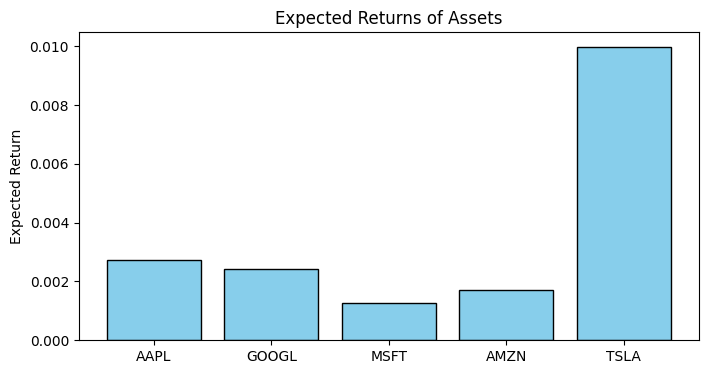
\includegraphics[width=0.45\textwidth]{mu.png}
        \hfill
        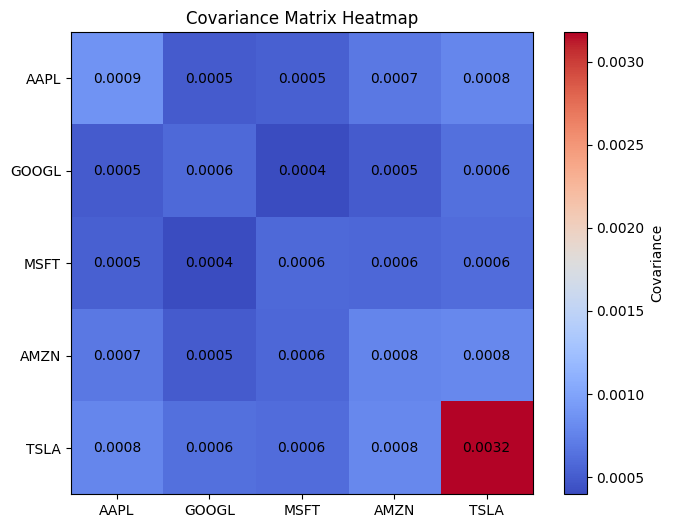
\includegraphics[width=0.45\textwidth]{sigma.png}
    \end{center}
\end{frame}

% Slide 5: Implementasi VQE dengan PennyLane
\section{Implementasi VQE}
\begin{frame}{Implementasi VQE dengan PennyLane}
    \begin{itemize}
        	\item \textbf{Framework:} PennyLane.
        \item \textbf{Ansatz:} 
        \begin{itemize}
            	\item Menggunakan \textit{Hardware-efficient ansatz} (\texttt{BasicEntanglerLayers}).
            	\item Kedalaman: 3 layer.
        \end{itemize}
        \item \textbf{Optimizer:} 
        \begin{itemize}
            	\item Gradient Descent Klasik untuk mengupdate parameter sirkuit.
        \end{itemize}
        \item \textbf{Proses:} Loop hibrid (Quantum Circuit $\leftrightarrow$ Classical Optimizer).
    \end{itemize}
    \vspace{0.3cm}
    \begin{center}
        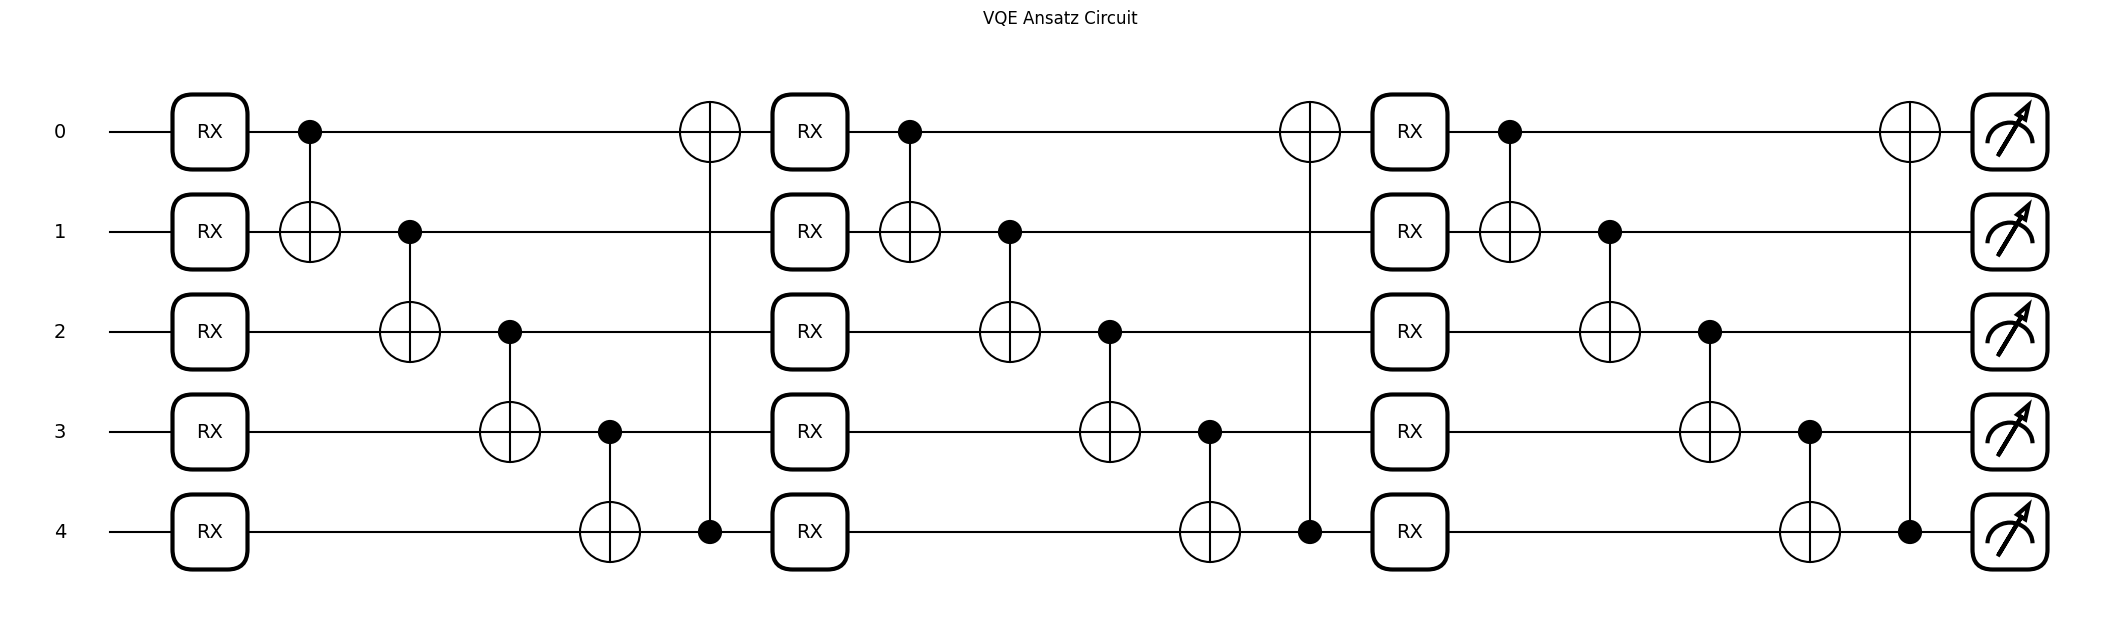
\includegraphics[width=0.7\textwidth]{Circuit.png}
        \hfill
        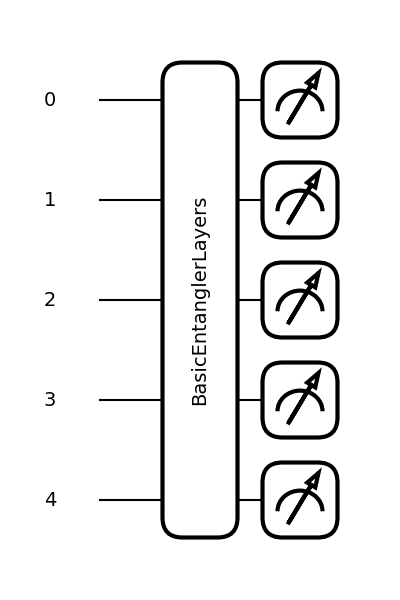
\includegraphics[width=0.225\textwidth]{circuit_visualization.png}
    \end{center}
\end{frame}

% Slide 6: Hasil Optimasi
\section{Hasil}
\begin{frame}{Hasil Optimasi}
    \begin{columns}
        \begin{column}{0.5\textwidth}
            \textbf{Grafik Konvergensi}
            \begin{itemize}
                	\item Penurunan nilai Cost function seiring iterasi (0 s.d 100).
            \end{itemize}
            \vspace{1cm}
            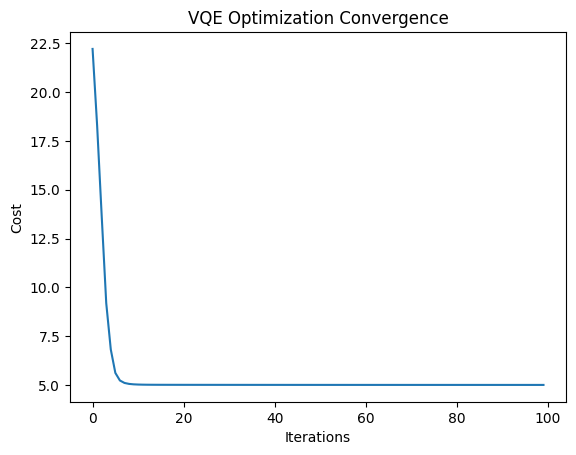
\includegraphics[width=\linewidth]{konvergensi.png}

        \end{column}
        \begin{column}{0.5\textwidth}
            \textbf{Hasil Akhir}
            \begin{itemize}
                	\item Probabilitas State Akhir tertinggi = Solusi Optimal.
                	\item \textbf{Optimal State:} \texttt{01001}
                	\item \textbf{Aset Terpilih:}
                \begin{itemize}
                    	\item GOOGL
                    	\item TSLA
                \end{itemize}
            \end{itemize}
        \end{column}
    \end{columns}
\end{frame}
\end{document}
